\section{Introduction}
% Logs are important. (But they can be forked breaking security guarantees of the apps using them. For example, CT logs. Recent work looks to Bitcoin due to its inherent resilience to forks. However, recent work is not efficient. Here we show how to do it efficiently.)
% ------------------
Security often depends on \emph{non-equivocation}\cite{frientegrity,coniks}.
For example, when a Certificate Authority (CA) equivocates by signing contradicting certificates for the same identity, it can impersonate websites and compromise users' privacy.
In fact, this has happened many times in the past\cite{cahacksurvey,cafrance,cahacks,caturkey,etisalat,mitmgoogle,certifiedlies}.
To prevent equivocation, Certificate Transparency (CT)\cite{ct} has been introduced as a way of publicly logging all CA-issued certificates.
However, a CT log server can still equivocate about the log of issued certificates and, together with a colluding CA, can launch impersonation attacks.
While gossiping\cite{ctgossip} about the log can help detect equivocation, detection can be slow or not happen at all, as gossip messages can be delayed indefinitely.
Another example is the Tor\cite{tor} anonymity network, where malicious directory servers can equivocate about the set of Tor relays and deanonymize users by tricking them to use malicious relays\cite{tortransparency}.
Thus, we believe non-equivocation is an important security requirement in many systems today, such as public-key distribution, blockchain-based transparency\cite{keybase,blockstack} and software transparency (see \secref{sec:background:motivation}).

% Fork-consistency is not enough
% ------------------------------
Unfortunately, without online trusted parties, achieving non\hyp{}equivocation is impossible\cite{sundrosdi}.
To deal with this impossibility result, systems resort to enforcing a weaker property called \emph{fork consistency}\cite{sundrosdi}.
Fork-consistent systems essentially make equivocation ``permanent'' and thus easier to prove later when clients are able to communicate or ``gossip'' out-of-band.
However, as illustrated above, for systems such as \pkds and Tor directory servers, undetected equivocation attacks can seriously impact users' security.
Thus, we believe a more proactive approach\cite{cosi} to security is desirable for such systems.

% Bitcoin witnessing is promising
% -------------------------------
To prevent equivocation proactively, recent work\cite{keybase,blockstack} uses the Bitcoin blockchain\cite{bitcoin}, as a witness.
We believe this \emph{Bitcoin witnessing} approach, though currently inefficient, is promising for three reasons.
First, this approach makes equivocation as hard as forking the Bitcoin blockchain itself, which has proven resistant to forking attacks.
Second, this approach only relies on a single global witness, namely the Bitcoin blockchain, obviating the need for users to obtain correct cryptographic identities of multiple trusted entities, such as log providers and auditors as in CT\cite{ct}, or witnesses as in CoSi\cite{cosi}.
It also has the advantage of not requiring the witness to keep any secrets, which if compromised would result in equivocation.
Third, the Bitcoin blockchain's open, decentralized and censorship-resistant nature makes deployment of witnessing schemes easy and interference with them hard.
Unfortunately, the main drawback of existing Bitcoin witnessing schemes has been that auditors have to download the entire Bitcoin blockchain, which, in November 2016, was almost \blockchainsize\cite{bitcoin-size} in size and growing by 52 GB every year.

% or t for top, b for bottom, h for here (https://tex.stackexchange.com/questions/35125/how-to-use-the-placement-options-t-h-with-figures)
\begin{figure}[t]
  \centering
    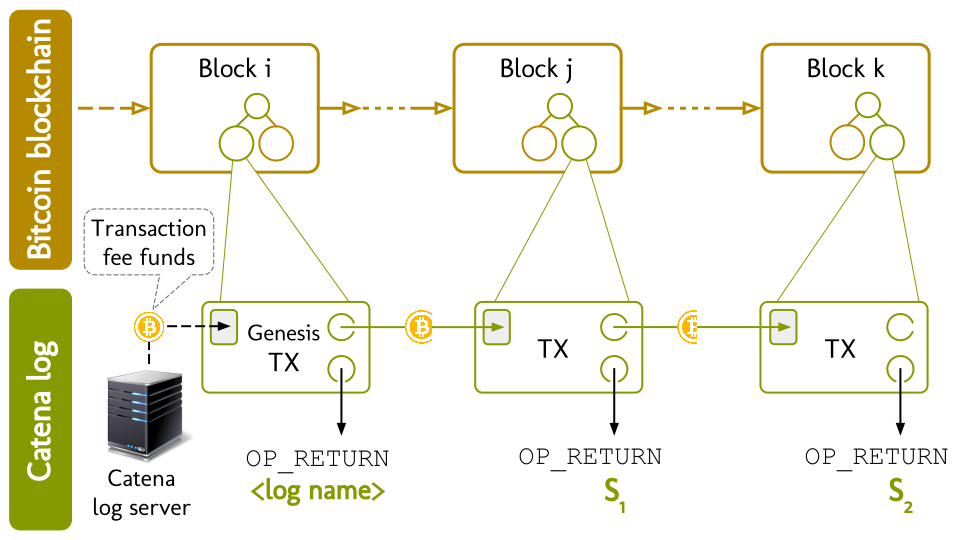
\includegraphics[width=1\columnwidth]{figs/overview.eps}
    \vspace{-.5cm}
    \caption{A \Sys log is a chain of Bitcoin transactions. Each \Sys transaction has two outputs: (1) a continuation output, which is spent by the next \Sys transaction, thus creating a chain and (2) an \opret output, which commits some application-specific statement. The server pays Bitcoin transaction fees for each issued statement. For applications that publish statements often, batching can be used to keep the fee per statement low.}
    \label{fig:catena-overview}
\end{figure}

% Elevator pitch
% --------------
This paper presents \emph{\Sys}, an efficient Bitcoin-based witnessing scheme that dramatically reduces auditors' bandwidth overhead.
At a high level, \Sys is a tamper-evident log\cite{ht} built on top of the Bitcoin blockchain.
\Sys prevents adversarial log servers who cannot fork the Bitcoin blockchain from equivocating about a log of application-specific statements.
Importantly, auditors who run \Sys clients can check the log for non-equivocation efficiently via Simplified Payment Verification (SPV)\cite{bitcoin} (see \secref{sec:background:bitcoin:thin}). 
This drastically decreases auditing bandwidth from \blockchainsize\cite{bitcoin-size} to only tens of megabytes, as \Sys clients only need to download Bitcoin block headers and small Merkle proofs under some of those headers.
Furthermore, after all block headers are downloaded, the bandwidth decreases to less than 1 KB of data every 10 minutes.


\subsection{Efficient Non-equivocation via Bitcoin}

Previous Bitcoin witnessing schemes\cite{keybase,blockstack} cannot \emph{efficiently} prove non-membership of inconsistent statements unless auditors download all the transactions in the Bitcoin blockchain.
Our design addresses this issue by allowing \Sys clients to skip downloading all irrelevant transactions while still guaranteeing non-equivocation.
\emph{The key idea behind \Sys is that Bitcoin's mechanism for preventing double spends can actually be regarded as a non-membership proof.}
Specifically, Bitcoin proves that no transactions double spending a previous transaction's output exist.
That is, if a client verifies blockchain membership for a transaction $tx_2$ which spends a previous transaction output $tx_1[0]$, that client has also implicitly verified that no other transaction $tx_2'$ which spends $tx_1[0]$ exists in the blockchain. ($tx_1[0]$ refers to the first output of transaction $tx_1$; see \secref{sec:background:bitcoin:transactions} for Bitcoin background.)

\Sys turns this idea into a non-equivocation scheme.
Each \emph{\Sys transaction} stores exactly one statement and spends the previous \Sys transaction, creating a chain of statements as shown in \figref{fig:catena-overview}.
This implies that if an auditor sees a statement $s_i$ in the blockchain whose transaction correctly spends the transaction for the previous statement $s_{i-1}$, then \emph{that constitutes a non-membership proof that no other inconsistent statement $s_i'$ exists}.
Looked at differently, if an adversarial log server wants to equivocate about $s_i$, it has to double spend the previous \Sys transaction for $s_{i-1}$, which can only be done by forking the Bitcoin blockchain.

\subsubsection{Root-of-Trust}
\Sys guarantees that once a client correctly obtains a log's \emph{genesis transaction}, the server cannot equivocate about that log unless it forks the Bitcoin blockchain.
The genesis transaction is the first transaction in the log and acts as the root-of-trust or ``\pk'' for a \Sys log (see \secref{sec:catena:design:genesis}).
Once clients obtain the correct genesis transaction they can efficiently verify that every issued statement comes from a transaction that spends coins originating from the genesis transaction.
In \secref{sec:catena:design}, we explain how this implicitly prevents equivocation in a \Sys log.
Our design is simple and efficient and obviates the need for log servers and clients to download the full Bitcoin blockchain while ensuring the consistency of the log.

\subsubsection{Bitcoin-friendly}
% Blockstack burns funds using a ``burn address.'' Not sure why they don't simply send the coins to the OP_RETURN output which commits their data.
To embed log statements in Bitcoin transactions, \Sys uses provably-unspendable \opret transaction outputs\cite{opreturn}, which, unlike previous work\cite{keybase-opret,blockstack}, does not harm Bitcoin by polluting the unspent transaction output (UTXO) set on Bitcoin nodes.
However, we emphasize that \Sys's novelty is not in leveraging \opret (previous work already does that; see \secref{sec:related-work}), but in chaining together \opret transactions that contain log statements, which makes it possible to check for non-equivocation efficiently.
Furthermore, \Sys does not place unnecessary stress on the Bitcoin P2P network.
First, clients query the \Sys log server directly to discover statements instead of using disk-intensive Bloom filtering on the Bitcoin P2P network (see \secref{sec:background:bitcoin:thin}).
Second, to avoid depleting the small connection pool of Bitcoin's P2P network, clients query a \emph{header relay network} (HRN) to obtain the latest Bitcoin block headers (see \secref{sec:catena:design:header-relay}).
Put simply, the HRN can be thought of as an ``extension'' of Bitcoin's P2P network for handling additional block header requests coming from \Sys clients.
We discuss potential attacks on the HRN in \secref{sec:attacks:hrn}.

\subsubsection{Applications}
Due to Bitcoin's 10-minute block rate, the \Sys log server can only issue a statement every 10 minutes while clients have to wait at least 60 minutes before accepting an issued statement.
Still, even with these delays, we believe \Sys can help secure applications such as key transparency schemes, Tor directory servers and software transparency schemes.
We discuss these applications in more detail in \secref{sec:background:motivation} and discuss \Sys's application-agnostic nature in \secref{sec:discussion:agnostic}.

\subsubsection{Evaluation}
To demonstrate the feasibility of \Sys, we implement a small-scale prototype in 3000 lines of Java using the bitcoinj Simplified Payment Verification (SPV) library\cite{bitcoinj} (see \secref{sec:prototype}).
Our current prototype does not include a Header Relay Network (HRN) so it will not scale to too many \Sys clients without stressing Bitcoin's P2P network.
We leave this to future work.
We also analyze the Bitcoin transaction fees the server has to pay per issued statement and show they could be anywhere between 7 to 12 US cents per statement.
Since existing systems like Keybase\cite{keybase} already pay close to 7 US cents per transaction, we believe this cost is practical.
Finally, we use our prototype to add Bitcoin witnessing to CONIKS\cite{coniks}, a recent key transparency scheme (see \secref{sec:prototype:coniks}), to demonstrate the ease of using \Sys.


\subsection{Contributions and Organization}

To summarize, this paper makes the following contributions:
\begin{itemize}
\item A new, \emph{efficient} approach to transparency based on witnessing in the Bitcoin blockchain.
\item \Sys, an append-only log built on top of Bitcoin that is efficiently verifiable by thin clients, obviating the need to download the full Bitcoin blockchain.
\item A prototype implementation of \Sys in Java that can be used by applications today.
\end{itemize}

\heading{Organization.} We motivate \Sys and present the Bitcoin background necessary to understand our design in \secref{sec:background}. We describe our system's actors, threat model and goals in \secref{sec:model}. We present \Sys's design in \secref{sec:catena:design} and we discuss attacks and countermeasures in \secref{sec:attacks}. We discuss our prototype implementation, its overheads and our extension of CONIKS in \secref{sec:prototype}.
We discuss remaining issues and future work in \secref{sec:discussion}.
We go over related work in \secref{sec:related-work} and we conclude in \secref{sec:conclusion}.


%\tableofcontents    % Comment me out please!

\section{Background and Motivation}
\label{sec:background}
In this section, we discuss our motivation for designing \Sys and give the necessary background on Bitcoin needed to understand \Sys's design.

\subsection{Motivation}
\label{sec:background:motivation}
Our main motivation for designing \Sys is to provide proactive security to many applications that depend on it.
At the same time, we want to improve previous blockchain-based transparency schemes\cite{keybase,virtualchain} whose shortcomings we describe in \secref{sec:background:motivation:blockchain-transparency}.
Finally, we want a non-equivocation scheme that does not require many trustworthy parties to come into existence and that can be deployed today.

\subsubsection{Key Transparency}
\label{sec:background:motivation:key-transparency}
% NOTE: Under their threat models (e.g., gossip works), they also prevent equivocation.
% .ECT: Section 2.2, page 3
% .DTKI: Section 6, page 12
% .CONIKS: Section 2.1, "Auditors", page 4
% .AKI: 
%   Section 4, page 3, Figure 1: browsers check roots against validators.
%   Section 2.2, page 2: non-collusion between CAs, log servers and validators. EFF is a validator.
% .ARPKI:
%   Section 4, page 4: Non-equivocation? (security) still holds even when n - 1 entities are compromised. Validators are optional (CAs are validators).
\Sys can prevent equivocation attacks in current key transparency work\cite{ct,ect,dtki,arpki,aki,coniks} and, as a result, thwart man-in-the-middle (MITM) attacks.
Key transparency schemes bundle public key bindings together into a directory implemented using authenticated data structures\cite{ad}.
Users are presented with digests of the directory as it evolves over time and can verify someone's \pk against a digest of the directory, preventing equivocation with respect to that digest.
The remaining problem for key transparency schemes is to prevent equivocation about the digests themselves.
For this, current schemes rely on federated trust\cite{coniks}, any-trust assumptions\cite{arpki}, non-collusion between actors\cite{arpki, aki} or on users gossiping between themselves\cite{ctgossip,ect,coniks,dtki} or with trusted validators\cite{aki}.

With \Sys, we propose using the Bitcoin blockchain as a hard-to-coerce, trustworthy witness that can vouch for directory digests.
For example, in Certificate Transparency (CT), a log server would directly witness \emph{signed tree heads} (STHs) in Bitcoin via a \Sys log.
Users can efficiently look up new STHs in the \Sys log and be certain that the log server has not equivocated about them.
We believe this approach could be more resilient to attacks, as a compromised log server cannot equivocate without forking the Bitcoin blockchain.
Also, because most transparency schemes publish digests of the directory periodically, we believe they are amenable to being secured by \Sys.

\subsubsection{Blockchain-based Transparency}
\label{sec:background:motivation:blockchain-transparency}
Blockchain-based transparency schemes\cite{keybase,blockstack} are promising due to their simplicity and resilience to forks, but the overhead of downloading all blockchain data makes them unusable on many devices.
\Sys can decrease the overhead of these schemes from currently \blockchainsize\cite{bitcoin-size} to around \headerssize.
For example, \Sys can enable thin clients running on mobile phones to efficiently audit the Bitcoin-witnessed Keybase \pkd\cite{keybase}.
Currently, Keybase publishes digests of their \pkd in Bitcoin by creating transactions signed by a predetermined \pk\cite{keybase-scheme}.
Keybase clients recognize these transactions and read directory digests from them (see \secref{sec:related-work} for details).
The problem with this approach is that thin clients cannot securely use Bloom filtering (see \secref{sec:background:bitcoin:thin}) to avoid downloading irrelevant transactions, as an adversary could selectively hide Keybase transactions and equivocate about the directory (we explain this attack in \secref{sec:catena:design:auditing}).
\Sys prevents this attack and also has the advantage of not polluting Bitcoin's unspent transaction output (UTXO) set\cite{keybase-opret}.

\Sys can also be used to improve Blockstack's thin client security \cite{blockstack}.
Currently, to benefit from Bitcoin's resilience against forks, Blockstack clients need to download the entire blockchain and compute their own \emph{consensus hash} over all Blockstack-related operations (see \secref{sec:related-work} for details).
Blockstack clients could also choose to trust someone else's consensus hash and verify \pk lookups against it efficiently using Simplified Name Verification (SNV)\cite{blockstack}.
However, clients still have to download full Bitcoin blocks to update that consensus hash or continue trusting someone else to update it.
As with Keybase, Bloom filtering cannot be used securely to filter Blockstack transactions.
To fix this problem, we propose using a \Sys log to keep track of Blockstack operations rather than scattering them through the blockchain.
In this way, thin clients can efficiently download just the Blockstack operations and quickly compute their own consensus hashes.

One disadvantage of this approach, according to one of the Blockstack co-founders\cite{blockstack-shea-jun-2016}, is that it requires a secret key to manage the \Sys log and would thus ``centralize'' the system.
To address this, an alternative design would be to introduce \emph{auditors} who verify and publish Blockstack consensus hashes in a jointly-signed \Sys log.
While this approach centralizes trust for thin clients, such as mobile phones, it does so in a more accountable and transparent manner.
Specifically, the auditors can't equivocate about consensus hashes but can still publish \emph{internally inconsistent}\cite{ht} consensus hashes (see \secref{sec:discussion:agnostic}).
However, such misbehavior would be evident in the Bitcoin blockchain when audited by a full Blockstack client.

\subsubsection{Software Transparency}
\Sys can prevent equivocation in \emph{software transparency} schemes\cite{software-transparency} and thus thwart man-in-the-middle attacks that try to inject malicious software binaries on victims' machines\cite{software-transparency}.
In fact, Bitcoin developers were concerned in the past about these kinds of attacks on Bitcoin binaries\cite{bitcoin-binary-transparency}.
To prevent these attacks, software vendors can publish digests of new versions of their software in a \Sys log.
Customers can then verify any version downloaded from a vendor's website against the vendor's log.
Previous work\cite{cosi} already highlights the necessity of software transparency in the face of insecure software update schemes\cite{secure-software-updates,attacks-on-package-managers}, key loss or compromise \cite{microsoft-golden-key} and black markets for code-signing certificates\cite{blackmarket-certs}.

\subsubsection{Tor Directory Servers}
\Sys can be used to prevent Tor directory servers\cite{tor} from equivocating about the directory of Tor relays.
Equivocation attacks are particularly concerning for Tor because they enable an attacker to easily deanonymize users by pointing them towards attacker-controlled Tor relays.
In fact, Tor Transparency\cite{tortransparency} plans to address these attacks by publicly logging the Tor directory consensus.
In the same spirit, we propose using \Sys to increase the resilience of Tor Transparency.
With \Sys, directory servers can publish the consensus in a \Sys log by jointly signing it using a Bitcoin multisignature\cite{multisig}.
Since Tor does not try to conceal who is connected to the network\cite{tor}, we are not concerned about \Sys's header relay network learning who is using Tor.
% If Tor users want to hide that they use Tor, they can rely on Tor bridges.
Finally, because Tor consensus is updated every hour, we believe it should be suitable for embedding in a \Sys log.

\subsubsection{Consensus Amongst $n$ Servers}
\Sys can be used by a set of $n$ servers to reach consensus on a log of operations, where each server manages its own secret key and does not necessarily trust the other $n-1$ servers.
In this scheme, each server submits an operation to the log by creating a \Sys transaction that is spendable by all $n$ servers (see \secref{sec:model:actors:log-server}).
To disincentivize the other servers from stealing the coins, the log is funded with small amounts of bitcoins and is frequently ``re-funded'' (see \secref{sec:catena:design:refund}).
This scheme allows all servers to reach consensus on the log and relies on Bitcoin miners to decide which server's operation gets included in the log.
To prevent adversarial servers from monopolizing the log with their operations by paying higher transaction fees, the servers can agree on an upper bound on fees.

%\subsubsection{Integrity-sensitive Systems}
%Verena, SUNDR\cite{sundrosdi}, SPORC. SPORC/SUNDR assume clients know each other's public keys (e.g., PKI) => clients can gossip securely and detect equivocation.

\subsection{Bitcoin Background}
\label{sec:background:bitcoin}

Bitcoin\cite{bitcoin,sokbitcoin,princetonbitcoinbook,bitcoinandbeyond} is a peer-to-peer digital currency that allows users to mint digital coins called \emph{bitcoins} and exchange them without a trusted intermediary.
Bitcoin uses a novel permissionless Byzantine consensus protocol known as \emph{proof-of-work consensus}\cite{blockchainproto} which allows all participants to agree on a log of transactions and prevent attacks such as double spending coins.
The log of transactions is called a \emph{blockchain} and is stored and managed by a peer-to-peer (P2P) network\cite{bitcoin-p2p}.
A special set of users called \emph{miners} run Bitcoin's proof-of-work consensus protocol, extending the blockchain with new \emph{blocks} made up of new transactions.
This process, called \emph{mining}, is computationally difficult and secures Bitcoin by allowing everyone to agree on the correct log of transactions while preventing Sybil attacks\cite{sybil}.
To incentivize Bitcoin miners to mine, a \emph{block reward} consisting of newly minted bitcoins is given to a miner if he mines or ``finds'' the next block.

\subsubsection{P2P Network}
\label{sec:background:bitcoin:p2p}
Bitcoin uses a peer-to-peer (P2P) network of volunteer nodes to store the blockchain\cite{bitcoin-p2p}, listen for new transactions or new blocks, and propagate this information throughout the network.
Users, such as merchants and their customers, download the blockchain by becoming part of the P2P network and can then receive or issue Bitcoin transactions.
Miners are also part of the P2P network where they listen for new blocks and broadcast their own blocks.

\subsubsection{Blockchain}
\label{sec:background:bitcoin:blockchain}
Bitcoin's ``blockchain'' is implemented as a hash-chain of \emph{blocks} (see \figref{fig:bitcoin}) and keeps track of all transactions in the system, allowing anyone to verify that no double spends have occurred.
A Bitcoin block is made up of a set of transactions (up to 1 MB) and a small \emph{block header} (80 bytes) that contains a hash pointer to the previous block.
The transactions in the block are hashed in a Merkle tree\cite{merkle} whose root hash is stored inside the block header.
The Merkle tree allows Bitcoin \emph{thin clients} (see \secref{sec:background:bitcoin:thin}) to obtain efficient \emph{membership proofs} that a transaction is part of a block.

% or t for top, b for bottom, h for here (https://tex.stackexchange.com/questions/35125/how-to-use-the-placement-options-t-h-with-figures)
\begin{figure}[t]
    \centering
    \includegraphics[trim=.8cm .8cm 1.4cm .8cm, width=1\columnwidth]{figs/bitcoin.pdf}
    \vspace{-1.5cm}
    \caption{The Bitcoin blockchain is a hash chain of blocks. Each block has a Merkle tree of transactions. Efficient membership proofs of transactions can be constructed with respect to the Merkle root. Here, $tx_1$ transfers coins from Alice, Bob and Carol to Dan and somebody else (miners receive a fee of 1 coin).
        Alice authorizes the transfer of her coins by signing $tx_1$, which has an input pointing to her coins locked in the 1st output of $tx_a$.
        Bob and Carol do the same.
        Similarly, Dan later spends his coins locked in $tx_1$'s 1st output by signing a new transaction $tx_d$ with an input pointing to $tx_1$'s 1st output.}
    \label{fig:bitcoin}
\end{figure}

\subsubsection{Decentralized Consensus}
\label{sec:background:bitcoin:consensus}
To solve the consensus problem in the decentralized or \emph{permissionless} setting, where participants can enter and leave the protocol as they please, Bitcoin introduces a novel Byzantine consensus protocol called \emph{proof-of-work consensus}\cite{blockchainproto,bitcoin-backbone,bitcoin-speed-security,miller2014anonymous}.
Though it does so at a high computational cost, this protocol defeats Sybil attacks\cite{sybil} and achieves consensus on the blockchain if 51\% of the computational power amongst participants remains honest.

Participants called \emph{miners} race to solve computationally-difficult proof-of-work puzzles derived from the previous Bitcoin block.
If a miner finds a solution, the miner can publish the next block by announcing it along with the solution (in reality, the solution is part of the next block) over the P2P network.
Furthermore, this miner will receive a \emph{block reward} in bitcoins, an incentive for miners to participate in the consensus protocol.
The puzzle difficulty is adjusted every 2016 blocks based on the inferred computational power of the miners, or \emph{network hashrate}, so that a new block is found or ``mined'' on average every 10 minutes.

When two miners find a solution at the same time, the Bitcoin blockchain is said to \emph{accidentally fork} into two chains.
In this case, Bitcoin peers use the \emph{heaviest chain rule} and select the heavier fork as the \emph{main chain} that dictates consensus.
The \emph{weight} of a fork is simply the amount of computational work expended to create that fork.
Assuming no difficulty changes, the heaviest fork is the longest fork.
However, across difficulty changes, it could be that a fork with fewer blocks is heavier than a longer fork (though this never happens in practice).

During an accidental fork, both forks have the same length and weight (assuming the fork does not cross a difficulty recomputation point), so Bitcoin peers adopt the fork they saw first as their main chain.
As more blocks are mined, one of the forks becomes heavier than the other and is accepted as the main chain by the whole network\cite{blockchainproto}.
In this case, the other abandoned fork and its blocks are said to be ``orphaned.''
In practice, accidental forks are infrequent and short: no more than one or two blocks get orphaned.
To deal with accidental but also with malicious forks, most Bitcoin nodes only consider a block and its transactions \emph{confirmed} if 6 or more blocks have been mined after it.

\subsubsection{Transactions}
\label{sec:background:bitcoin:transactions}
Bitcoin transactions facilitate the transfer of coins between users (see \figref{fig:bitcoin}).
A Bitcoin transaction has an arbitrary number of \emph{transaction inputs}, which authorize the transfer of coins, and \emph{transaction outputs} (TXOs), which specify  who receives those coins and in what amounts.
Naturally, the number of coins locked in the outputs cannot exceed the number of coins specified in the inputs (with the exception of so-called ``coinbase'' transactions, which mint new coins and have no inputs).
A transaction output specifies an amount of coins and their new owner, most commonly as a \pk.
A transaction input refers to or ``spends'' a previously unspent transaction output (UTXO) and contains a proof-of-ownership from that UTXO's owner, which authorizes the transfer of those coins.
For the purposes of this paper, we only make use of the case where outputs specify owners using \pks and inputs prove ownership using signatures.

Importantly, when assembling transactions into blocks, Bitcoin miners prevent double spends by ensuring that, across all transactions in the blockchain, for every TXO there exists at most one transaction input that refers to or spends that TXO.
This invariant is known as the \emph{TXO invariant} and \Sys leverages it to prevent forks.
Finally, a transaction's fee is the difference between the coins spent in its inputs and the coins transferred by its outputs.
The fee is awarded to the miner who mines a block containing that transaction.
In theory, the fee can be zero, but in practice recent contention for space in the blockchain requires users to pay transaction fees.

\subsubsection{Storing Data in Transactions}
\label{sec:background:bitcoin:opret}
Bitcoin allows users to store up to 80 bytes of data in transactions through provably-unspendable \opret transaction outputs.
Importantly, any coins specified in the output are forever unspendable or ``burned''.
For simplicity, \Sys uses \opret outputs to store application-specific statements in the Bitcoin blockchain (see \secref{sec:catena:design}).
However, there are other ways to store data in Bitcoin transactions: in the value of transferred coins\cite{bitcoin-storing-data}, in transaction inputs \cite{bitcoin-p2sh-data}, in transaction sequence numbers\cite{bitcoin-storing-data}, or in an output's \pk (either via vanity \pks\cite{bitcoin-storing-data}, fake \pks\cite{keybase-scheme}, multisig \pks\cite{multisig} or ``pay-to-contract'' \pks\cite{bitcoin-pay-to-contract}).

\subsubsection{Thin Nodes vs. Full Nodes}
\label{sec:background:bitcoin:thin}
Bitcoin's P2P network is made up of \emph{full nodes}, which download the entire blockchain and validate all the transactions (see \secref{sec:background:bitcoin:p2p}) and \emph{thin nodes}, which only download small 80 byte block headers and cannot fully validate transactions.
Since full nodes are more expensive to run (higher bandwidth, computation and space), smaller devices such as smartphones can run thin nodes instead, also known as \emph{Simplified Payment Verification} (SPV) nodes.

Thin nodes verify Bitcoin transactions more efficiently under a slightly stronger assumption about the Bitcoin network.
A thin node considers a transaction valid if it sees a correct Merkle proof of membership for that transaction in a block.
Furthermore, the more blocks are mined after a transaction's block (also known as \emph{confirmations}), the more confident a thin node can be that the transaction is indeed valid.
Importantly, thin nodes don't even verify signatures on transactions: the membership proof coupled with enough confirmations offers enough assurance that the transaction was verified by miners and is thus valid.
As a result, thin nodes assume Bitcoin miners follow their incentives and create correct blocks or otherwise thin nodes could accept invalid transactions.
This assumption can be reasonable since miners would lose their block reward if they create invalid blocks (see \secref{sec:background:bitcoin:consensus}).

Finally, the only way for thin nodes to avoid downloading unnecessary data is to use a Bitcoin feature called Bloom filtering\cite{bitcoin-bloom}.
This feature allows thin nodes to only receive transactions of interest by asking remote peers to filter out irrelevant transactions using a Bloom filter\cite{bloom}.
Bloom filtering is cheap for the requesting thin client but quite expensive for the servicing full node, which has to load all requested blocks from disk, pass them through the filter and send filtered blocks to the thin client.

\section{Model and Goals}
\label{sec:model}
In this section we describe our system actors, our threat model and our design goals.

\subsection{Actors}
\label{sec:model:actors}
The main actors in our scheme are the log server, which appends statements to the log, \Sys clients, which verify new statements and check for non-equivocation, and the header relay network (HRN), which helps scale \Sys to support a large number of clients (see \figref{fig:communication}).

\subsubsection{Log server}
\label{sec:model:actors:log-server}
A log server manages an append-only log of application-specific \emph{statements}.
The log server appends statements to the log by signing Bitcoin transactions with statement data embedded in them and broadcasting them to the Bitcoin P2P network.
We call these transactions \emph{\Sys transactions} and defer their discussion to \secref{sec:catena:design:transactions}.
In this paper, we will mostly talk about a single log server managing the log, but by using Bitcoin multisignatures\cite{multisig}, \Sys can support multiple servers who either jointly or separately append statements to the log.
Also, although a log server can manage many different logs, for simplicity we restrain our discussion to a single server managing a single log.

\subsubsection{Clients}
Multiple clients connect to the log server and keep up with new log statements.
As depicted in \figref{fig:communication}, clients fetch \Sys transactions from the log server and verify they have been included in the Bitcoin blockchain.
This verification is done against block headers obtained from the header relay network (discussed next).
\Sys clients want to prevent log server equivocation: a client who is shown a statement $s_i$ wants to ensure there is no other contradictory statement $s_i'$ in the log at position $i$ (see \secref{sec:model:goals:noneq}).

\subsubsection{Header Relay Network}
Due to the low connection capacity of the Bitcoin P2P network (see \secref{sec:catena:design:header-relay}), \Sys clients use a separate header relay network (HRN) to obtain Bitcoin block headers (see \secref{sec:catena:design:header-relay}).
Otherwise, \Sys would put unnecessary stress on Bitcoin's P2P network and would not scale well.

\newcommand{\api}{\hangindent=\parindent \hangafter=1 \noindent}
\newcommand{\createlog}{\mathsf{CreateLog}\xspace}
\newcommand{\appendstmt}{\mathsf{AppendStmt}\xspace}
\newcommand{\verifystmt}{\mathsf{VerifyStmt}\xspace}
\newcommand{\txgen}{\mathsf{tx}_{\textsf{genesis}}}

\subsection{\Sys API}
\label{sec:model:api}

Our scheme can be succinctly described as a tuple $\langle \createlog, \appendstmt, \verifystmt \rangle$ of API calls.
For clarity, we prefix calls with $S$ when they are made by the log server and with $C$ when they are made by clients.
\\

\api $S.\createlog(d) \rightarrow (\sK, \pK)$.
Creates an empty log. 
All future log statements can be verified against the log's public key $\pK$.
Embeds some arbitrary data $d$ in the log (e.g., the log's name).

\api $S.\appendstmt(\sK, s_i)$.
Appends the statement $s_i$ to the log, signing it using $\sK$.

\api $C.\verifystmt(\pK, i, s_i) \rightarrow \{\mathsf{True, False}\}$.
Verifies that the statement $s_i$ is contained in the log with \pk $\pK$ at position $i$.
Returns true if successful or false otherwise.
Before being called on $s_i$, $\verifystmt$ must first be called on $s_1, s_2, \dots, s_{i-1}$, in that order.
\\

To recap, a server creates a new log by calling $\createlog$ and appends statements to this log using $\appendstmt$.
Clients verify each new statement $s_i$ by calling $\verifystmt$ in order for $i = 1, 2, 3, \cdots$.

\subsection{Threat Model}
\label{sec:catena:threat-model}
% Previous work assumptions:
% .CT: Not stated specifically, but they assume STH-gossiping, trusted monitors and trusted auditors.
% .ECT: Malicious-but-cautious; can mount active attacks but only if he stays undetected. One assumption seems to be the adversary cannot equivocate because gossiping will detect it.
% .CONIKS: Does not mention anything about "network", "active" or "passive" adversaries. Assumes a PKI for providers. Providers can deter each other from equivocating.
% .AKI: CAs, public logs and validators do not collude. Browsers have their PKs (like a small PKI). Adversary can gain control of some but not all the servers the user trusts. Adversary can gain control of all servers that the user does NOT trust.
% .ARPKI: Active adversary can drop, modify, insert messages at will (to a certain extent), but he cannot compromise keys of certain actors (only n-1 out of n can be compromised).

% Server can equivocate
% ---------------------
\subsubsection{Adversarial Log Server}
\label{sec:model:threat:log-server}
We assume the \Sys log server is compromised or coerced and wants to equivocate about statements.
We assume \Sys clients can correctly obtain the log's genesis transaction which acts as the log's ``public key'' (see \secref{sec:catena:design:genesis}).
We note that both \Sys and previous work\cite{ct,ect,coniks,aki,arpki,cosi} all rely on some sort of initial public-key distribution.
However, unlike previous work, \Sys can prevent equivocation once a client has the ``public key'' or genesis transaction.
It's important to understand that, similarly to how a signature can only be verified with respect to a public key, equivocation can only be prevented with respect to a log identified by some kind of information, in this case, the genesis transaction.

We stress that \Sys's goal is to prevent equivocation given a log's genesis transaction and orthogonal techniques can be used for distributing the genesis transaction.
For instance, the log's genesis transaction can be shipped with the application software that audits that log, similar to how browsers are shipped with public keys of Certificate Authorities (CAs).
In fact, we argue it might be easier for end-users to verify the genesis transaction if they know the log's creation date.
Specifically, users can download just the blocks around that date and check that no other genesis transaction for the log exists in those blocks.

% Proof-of-work consensus
% -----------------------
\subsubsection{Proof-of-Work Consensus}
\label{sec:model:threat:pow}
Similar to previous work \cite{virtualchain, blockstack, keybase, bitcoin-smc, bitcoin-anon-cred, versum, bitcoin-incent-comp, bitcoin-pred-mkt,commitcoin}, we assume that adversaries cannot break Bitcoin's proof-of-work consensus and fork the blockchain.
Specifically, we assume that a \Sys transaction is immutable once it has been confirmed by a sufficient number of blocks, as configured by \Sys clients individually (we recommend at least 6 blocks).
We believe it is reasonable to assume that long malicious forks are unlikely to occur due to the computational difficulty and financial burden of such an attack.
We also assume the \Sys log server cannot collude with large Bitcoin miners, who are not likely to benefit financially from a forking attack.
Finally, we have to assume Bitcoin's P2P network is reliable and miners hear about each other's blocks quickly, or else proof-of-work consensus could be easily subverted\cite{blockchainproto,eclipse}.
We discuss attacks on Bitcoin's consensus in more detail in \secref{sec:attacks}.


% or t for top, b for bottom, h for here (https://tex.stackexchange.com/questions/35125/how-to-use-the-placement-options-t-h-with-figures)
\begin{figure}[t]
    \centering
    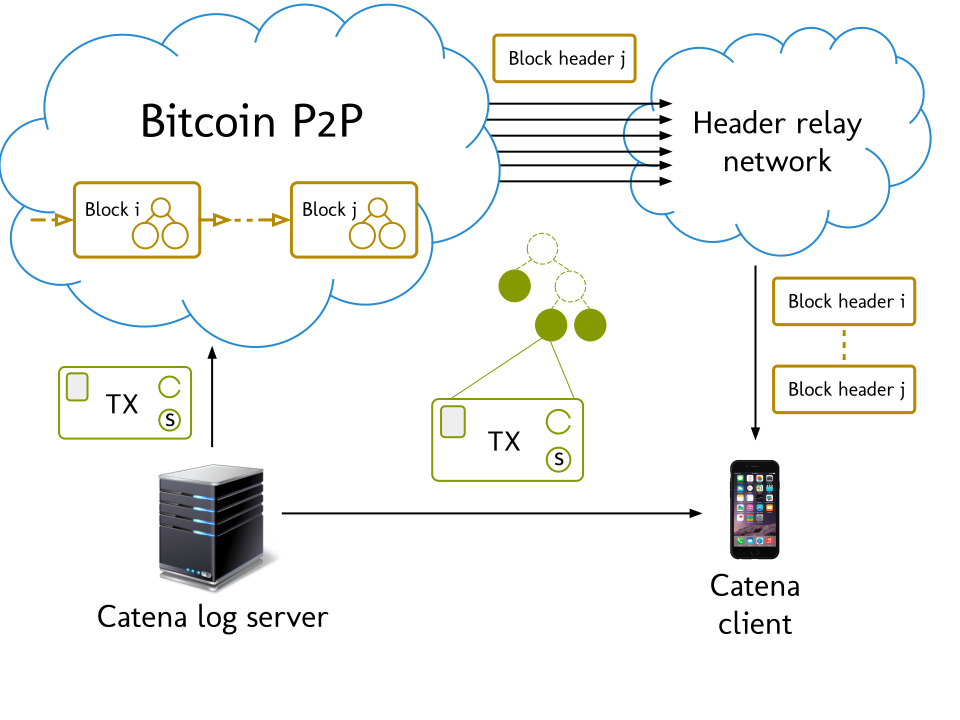
\includegraphics[width=1\columnwidth]{figs/communication.eps}
    \vspace{-1.2cm}
    \caption{The log server broadcasts \Sys transactions with statements embedded in them to the Bitcoin P2P network. \Sys clients query the header relay network for block headers and the log server for statements with proofs they were witnessed in the Bitcoin blockchain. The header relay network maintains good connectivity to the Bitcoin P2P network without depleting the P2P network's connection pool.}
    \label{fig:communication}
\end{figure}

% Thin client assumption
% ----------------------
\subsubsection{SPV Assumption}
\Sys clients use thin nodes (see \secref{sec:background:bitcoin:thin}) to efficiently verify the log for non-equivocation.
It's important to note that thin nodes are less secure than full nodes against adversarial mining attacks (see \secref{sec:attacks:adversarial-mining}).
Also, thin nodes have to assume miners verify their own blocks and the blocks of other miners before mining, otherwise thin nodes risk accepting invalid transactions.
Fortunately, Bitcoin miners have a strong incentive to verify blocks, as they would lose the block reward if they extend an invalid blockchain.
However, recent work\cite{consensuscomputer} shows that when block verification is expensive miners have an incentive to skip it.
We discuss such an event that occurred in 2015 in \secref{sec:attacks:accidental-forks}.

\subsubsection{Header Relay Network}
% This network is open => Sybil attacks => eclipse attacks => easier generalized Vector76 attacks / Finney attacks (but we discuss defenses later)
% This network is NOT open => contradicts our motivation about requiring trustworthy parties to come into existence
We trust \Sys's header relay network to serve \Sys clients with the latest Bitcoin block headers.
Similar to a compromised Bitcoin P2P network, a compromised HRN can eclipse\cite{eclipse} \Sys clients and help adversaries win mining races faster and thus equivocate (see \secref{sec:attacks:adversarial-mining}).
However, such adversaries would need a significant fraction of mining power to win races fast enough without \Sys clients noticing they are being eclipsed.
We discuss such attacks in \secref{sec:attacks:hrn}.

\subsection{Goals}
\label{sec:catena:goals}
Our goals are to prevent equivocation and to do so in an efficiently-verifiable manner, enabling each user to audit individually and thus minimizing trust in applications such as \pkds.

\subsubsection{Non-equivocation}
\label{sec:model:goals:noneq}
A log server should have a hard time equivocating about log statements.
\Sys makes equivocation in the log as hard as forking the Bitcoin blockchain, which we believe to be a reasonable amount of protection for many applications, including \pkds.
If our assumptions are broken and the Bitcoin blockchain forks, \Sys cannot prevent equivocation but still makes equivocation detectable once the forks are resolved, similar to previous gossip-based approaches\cite{ctgossip,ect,coniks,dtki}.

% Clarification about why equivocation is problematic
% ---------------------------------------------------
It's important to understand what non-equivocation actually provides.
Non-equivocation does not prevent the adversarial log server from issuing incorrect statements that break semantics at the application layer.
Instead, non-equivocation simply guarantees that all clients see all issued statements, including incorrect ones.
This allows clients to detect attacks at the application layer, as we discuss later in \secref{sec:discussion:agnostic}.

\subsubsection{Publicly Verifiable}
Given a log's genesis transaction $\txgen$ (i.e., its \pk), anyone can verify the full history of statements in that log.
Specifically, a client can obtain all statements $\langle s_1, s_2, \dots, s_n \rangle$ in the log and verify them with respect to $\txgen$.
Verification here means that a statement is part of the log at some position $i$ and no other inconsistent statement at position $i$ exists (\ie non-equivocation).
In particular, for any statement $s_i$, the log server gives the client a publicly verifiable proof $p$ with respect to the log's $\txgen$ that proves that $s_i$ is indeed the only statement in the log at position $i$.

\subsubsection{Efficiently Verifiable}
\label{sec:catena:goals:efficiency}
\Sys clients should be able to audit logs efficiently without downloading the entire Bitcoin blockchain.
Recent blockchain-based transparency work\cite{keybase,blockstack,coniks} is inefficient, requiring auditors to download the entire blockchain to prevent equivocation (see \secref{sec:background:motivation:blockchain-transparency}).
This raises the barrier to entry for log auditors, who might have to outsource auditing or trust the log blindly.
In contrast, the barrier for \Sys clients is very low: clients only download 80-byte block headers for each Bitcoin block and 600-byte Merkle membership proofs for each statement (see \secref{sec:catena:design:auditing}).


\section{\Sys Design}
\label{sec:catena:design}

At a high level, \Sys makes equivocation about a log statement as hard as double spending a Bitcoin transaction output.
The key idea behind \Sys is to embed statements in Bitcoin transactions and have each transaction spend the previous one.
This is a simple but powerful idea because \emph{it forces the log server to double spend a transaction output if it wants to equivocate}, which is notoriously difficult in Bitcoin.
Thus, \Sys can offer a strong guarantee to clients that they have not been equivocated to.

\Sys operates very simply, as illustrated in \figref{fig:catena-overview}.
The \Sys log server creates a log by issuing an initial transaction called the \emph{genesis transaction}.
The server issues the first statement in the log by creating a new transaction that spends the genesis transaction and commits that first statement via an \opret transaction output (see \secref{sec:background:bitcoin:opret}).
Finally, the server can append new statements to the log by  creating a new transaction that spends the previously-created transaction and commits a new statement.

\Sys clients first obtain the log's genesis transaction, which can be shipped with the higher-level application that \Sys secures (see \secref{sec:model:threat:log-server}).
Then, clients obtain and verify all Bitcoin block headers from the header relay network (discussed in \secref{sec:catena:design:header-relay}).
Finally, clients can ask the \Sys log server for the statements and verify them against the genesis transaction and the Bitcoin block headers.
Importantly, because \Sys transactions are ``chained'' (see \figref{fig:non-equivocation}) and Bitcoin prevents double spends, clients are assured the server has not equivocated (see \secref{sec:model:goals:noneq}).

\Sys's overhead is small.
For each 32-byte statement, the server sends over a 235-byte \Sys transaction and a Merkle path of up to 350 bytes proving that the statement is part of the log.
That amounts to around 600 bytes per statement plus the overhead of downloading all block headers (currently \headerssize), making \Sys very cheap in terms of bandwidth.

% Avg # of TXs is 2000 nowadays. Each proof is 256 bits * log_2(2048) = 256 bits * 11 = 352 bytes. 
% https://blockchain.info/charts/n-transactions-per-block?timespan=all 
%
% Each OP_RETURN TX with a 32-byte payload is 235 bytes => Proof + TX = 235 + 352 =~ 600 bytes
% https://tradeblock.com/bitcoin/tx/8bae12b5f4c088d940733dcd1455efc6a3a69cf9340e17a981286d3778615684 (not sure why this is >250 bytes)
% https://blockchain.info/tx/29c108fbbf672fac9536aa25ae7f3931c9588a0e10650c73ff5883531af2ef45?show_adv=true (235 bytes as expected)
% https://tradeblock.com/blog/analysis-of-bitcoin-transaction-size-trends (average block is around 2000 TXNs)


\subsection{Transaction Format}

\subsubsection{Genesis transaction}
\label{sec:catena:design:genesis}
\Sys logs are identified by a genesis transaction.
This is the first transaction created by the log server when it starts the log.
The genesis transaction effectively acts as the log's ``\pk'': once a client has the log's genesis transaction, that client can verify log updates against it and prevent equivocation.
As discussed in \secref{sec:model:threat:log-server}, a ``\pk'' such as the genesis transaction is a necessary element of any system which aims to prevent equivocation.

\subsubsection{\Sys transactions}
\label{sec:catena:design:transactions}
A \Sys log is just a chain of specially-crafted Bitcoin transactions called \emph{\Sys transactions} (see \figref{fig:catena-overview}).
Our transaction format is simple.
First, a \Sys transaction has one input, which spends the previous \Sys transaction in the chain, and extra inputs for ``re-funding'' the log (see \secref{sec:catena:design:refund}).
Second, a \Sys transaction has two outputs.
The first output is an unspendable \opret output, which commits the log statement, and the second output is a \emph{continuation output}, which is spent by the next \Sys transaction's input.
The genesis transaction also has the same \Sys transaction format.

% or t for top, b for bottom, h for here (https://tex.stackexchange.com/questions/35125/how-to-use-the-placement-options-t-h-with-figures)
\begin{figure}[t]
	\centering
	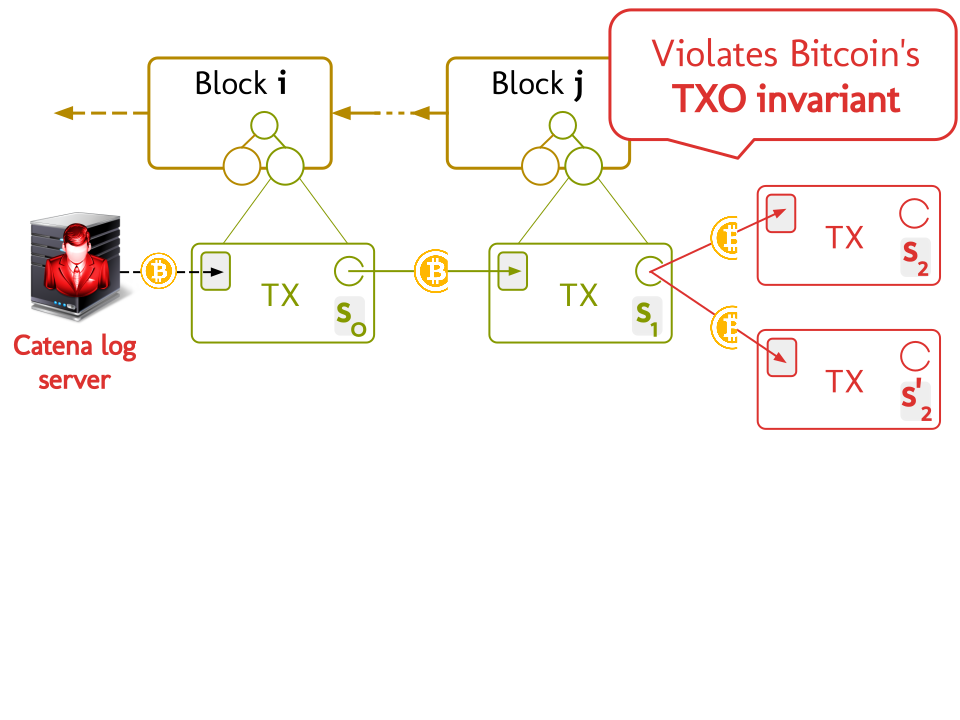
\includegraphics[width=1\columnwidth]{figs/non-equiv.pdf}
	\vspace{-3.2cm}
	\caption{Equivocating in a \Sys log is as hard as double spending in Bitcoin, which requires forking the blockchain (see \secref{sec:background:bitcoin}). This is because \Sys's design requires a new \Sys transaction to spend the previous one, which linearizes the history of statements embedded in those transactions.}
	\label{fig:non-equivocation}
\end{figure}

% Transaction format prevents equivocation
% ----------------------------------------
Our transaction format leverages the fact that Bitcoin miners prevent double spends which, in turn, allows us to prevent equivocation about statements (see \figref{fig:non-equivocation}).
The key idea is that a \Sys transaction has a single spendable output, which means Bitcoin miners will ensure \emph{only a single future transaction spends that output} (see TXO invariant in \secref{sec:background:bitcoin:transactions}).
Thus, a \Sys transaction can only be followed by another \emph{unique} \Sys transaction, which allows us to create a linear history of statements that all \Sys clients can agree on.

% Statement key
% -------------
\Sys transactions just transfer coins from the \Sys log server back to itself, committing log statements and paying fees to Bitcoin miners in the process.
Recall from \secref{sec:background:bitcoin:transactions} that a transaction output specifies a coin amount and a public key that ``locks'' those coins (\ie is authorized to spend them later).
In \Sys, all transaction outputs are locked by the same key called the \emph{statement key}, which is managed by the log server.
This key signs all \Sys transactions, including the statements embedded in them, authorizing the transfer of coins back to the server.
\Sys clients can easily obtain the statement key from the genesis transaction since it is specified in its continuation output.
% (In practice, they obtain the key's fingeprint/address from the genesis transaction's continuation output and the actual PK from the next TXN's input.)
The server can change the statement key in future transactions and clients can easily pick up the new key, but for simplicity we assume it remains the same across all \Sys transactions.

% Transaction fees
% ----------------
As mentioned before, the log server has to pay fees to Bitcoin miners to get its transactions included in the blockchain.
We describe how this works in \secref{sec:catena:design:refund} and we analyze the server's cost per \Sys statement in \secref{sec:prototype:fees}.


\subsection{Header Relay Network}
\label{sec:catena:design:header-relay}
We want to avoid stressing Bitcoin's P2P network, which has a limited connection capacity that would be quickly depleted by \Sys clients.
There are currently around 5500 full Bitcoin nodes, each by default capable of handling up to 117 incoming connections\cite{bitcoin-bitnodes-21co,bitcoin-p2p}.
Thus, Bitcoin's P2P network currently supports at most 643,500 incoming connections at a single point in time, some of which are already used up by Bitcoin thin clients for user wallets.
Importantly, these connections need to be long-lived so as to allow \Sys clients to discover and connect to a diverse set of Bitcoin peers.
As a result, if each \Sys client were to maintain 8 outgoing connections to Bitcoin's P2P network, then \Sys would not scale beyond tens of thousands of clients without putting significant stress on the Bitcoin network.

To provide scalability, we propose using a header relay network (HRN) that is well connected to the Bitcoin P2P network and can serve block headers to hundreds of thousands of \Sys clients.
An HRN node operates as a full node in the Bitcoin P2P network, contributing to its health while providing an interface to \Sys clients for obtaining block headers fast.
However, note that HRN nodes do not mine nor attempt to reach consensus on block headers: they just gossip and verify blocks like the rest of the Bitcoin P2P network.
\Sys clients trust the HRN to serve them with the latest Bitcoin block headers.
Importantly, clients ask multiple HRN nodes for block headers to ensure they are not being eclipsed by a single malicious HRN node.
We discuss attacks on the HRN in \secref{sec:attacks:hrn}.

% Boootstrapping HRNs
% -------------------
A header relay network can be bootstrapped in various ways.
The simplest way is to have a set of volunteer HRN nodes that act as an extension of the Bitcoin P2P network.
Another way is to rely on current blockchain explorers\cite{bitcoin-blockchaindotinfo, bitcoin-blockexplorerdotcom, bitcoin-blockrdotio,bitcoin-blocktraildotcom} since they are well connected to the Bitcoin network and already provide public APIs for fetching block headers.
A diverse HRN could be implemented by publishing block headers across various websites, such as Twitter, Facebook or GitHub, in a publicly-verifiable manner similar to how Keybase\cite{keybase} users publish identity proofs.
A peer-to-peer HRN can be bootstrapped amongst \Sys clients themselves.
\Sys clients can occasionally fetch block headers from the Bitcoin P2P network and then distribute them amongst themselves.
To avoid stressing Bitcoin P2P nodes, each client would query the Bitcoin P2P network with probability inversely proportional to the size of HRN (estimated using known techniques\cite{p2p-size-estimation}).
Finally, Sybil attacks\cite{sybil} in all these types of HRNs can be addressed by requiring HRN nodes to ``burn'' bitcoins in a publicly-verifiable manner (see \secref{sec:background:bitcoin:opret}) and tie their identity to those burned coins.

% https://bitcoin.stackexchange.com/questions/37344/is-the-spv-client-model-scalable
% At best, if a full node can read blocks at 20MB/s from disk and filter them with close to no overhead, it would only be able to send 20 filtered blocks per second.
% With 5500 nodes in the network, in an ideal world, this would amount to a total available bandwidth of 110,000 filtered blocks per second.
% However, a full node's throughput in terms of block headers/sec is quite high: easily serve 100,000 headers/sec to a single client and more to multiple clients.
% \Sys nodes add close to no overhead to Bitcoin nodes, requiring little time to sync up: a few seconds for downloading \headerssize of block headers.


\subsection{Auditing a \Sys Log}
\label{sec:catena:design:auditing}
% Overview of auditing
% ---------------------
To audit a log, clients download the \Sys transaction chain and verify that transactions are signed and spend each other correctly using the statement key.
Clients first download and verify block headers from the header relay network and then download and verify \Sys transactions and their Merkle proofs from the log server.
This way, \Sys clients avoid Bloom filtering on Bitcoin's P2P network, which causes significant disk activity for full nodes (see \secref{sec:background:bitcoin:thin}).
Finally, auditing is cheap for \Sys clients as they only download small transactions and Merkle proofs (600 bytes) and not full Bitcoin blocks (1 MB).

% Verifying a transaction
% -----------------------
To verify a new \Sys transaction $tx_i$, a client checks that:
\begin{enumerate}
\item $tx_i$ is in the correct \Sys format.
\item $tx_i$ is correctly included in a Bitcoin block with a Merkle membership proof.
\item The first input of $tx_i$ spends the continuation output of the previous \Sys transaction $tx_{i-1}$.
\item $tx_i$ is signed correctly with the statement key of the log.
\item $tx_i$ has a sufficient number of confirmations (we recommend at least 6).
\end{enumerate}

% Checking transaction signatures
% -------------------------------
It's important to understand that without clients verifying transaction chaining (\ie step 3 and 4 above), a malicious log server can equivocate about statements in the log.
For example, consider two \Sys clients $c_1$ and $c_2$ which correctly obtain the genesis transaction $\txgen$ of the log but do not verify transactions are chained.
In this attack, the malicious log server issues two \Sys transactions that commit two different statements $s_1$ and $s_1'$ respectively but, importantly,  \emph{do not spend} the genesis transaction.
Instead they spend some other transactions and get included in the blockchain.
The attack is straightforward: the log server shows client $c_1$ the transaction for $s_1$ but hides the one for $s_1'$.
Similarly, it shows client $c_2$ the transaction for $s_1'$ and hides the one for $s_1$.
As a result, the log server can easily equivocate to clients who don't verify transaction chaining as they cannot ensure the server is not hiding an inconsistent statement.
To conclude, in \Sys, clients prevent this attack by checking that every statement they accept is part of a transaction that spends the previous transaction's continuation output, chaining all the way back to the genesis transaction.


\subsection{Blockchain Reorganizations}
\label{sec:catena:design:reorgs}
Like Bitcoin, \Sys also needs to deal with small day-to-day accidental forks or \emph{blockchain reorganizations} (see \secref{sec:background:bitcoin:consensus}).
These small forks are automatically resolved by the Bitcoin network: as more blocks are found, eventually one of the forks overtakes the other one and becomes the main chain\cite{blockchainproto}.
To be certain payments are not reversed by these small reorganizations, Bitcoin merchants only consider a block and its transactions confirmed if 6 or more blocks are built on top of it.

\Sys also allows clients to set their own application-specific number of required confirmations before accepting a statement (a minimum of 6 is recommended).
As a result, \Sys makes a trade-off between resilience to forks and latency of accepting statements.
Additionally, as a security measure against longer accidental forks, \Sys clients remember recently-issued statements.
This way, if a statement is withdrawn due to a reorganization, \Sys clients can ensure the reissued statement matches the previously seen one.


\subsection{Paying for a \Sys Log}
\label{sec:catena:design:refund}
A \Sys log server must pay Bitcoin transaction fees to start a log and append statements to it.
Initially, the \Sys log server must obtain some bitcoins (BTC), perhaps from a Bitcoin exchange\cite{bitcoin-exchanges}.
Then, the server can issue the log's genesis transaction and pay for its fee.
The server locks some coins in the genesis transaction's continuation output which can ``fund'' future log transactions.
To issue the first statement, the server signs a new \Sys transaction with the statement key.
This transaction commits the statement (via an \opret output), transfers the genesis transaction's coins back to the log server and leaves a small fee for the miners.
As before, the remaining coins are locked in this new transaction's continuation output.
The server repeats this process for every new statement, spending the coins locked in the previous \Sys transaction, until it runs out of funds.
We analyze the costs of running a \Sys log in terms of transaction fees in \secref{sec:prototype:fees}.

% or t for top, b for bottom, h for here (https://tex.stackexchange.com/questions/35125/how-to-use-the-placement-options-t-h-with-figures)
\begin{figure}[t]
	\centering
	\includegraphics[width=1\columnwidth]{figs/refunding.pdf}
	\vspace{-3.1cm}
	\caption{A \Sys chain can be ``re-funded'' by allowing the next transaction in the chain to have additional inputs that lock extra coins in that transaction's continuation output. In this example, \Sys transactions pay .5 BTC as a fee so to ensure $tx_8$ does not run out of coins we ``re-fund'' it using extra inputs.}
	\label{fig:refunding}
\end{figure}

To ``re-fund'' the chain, \Sys transactions can have additional inputs that lock extra coins in that transaction's continuation output (see \figref{fig:refunding}).
Importantly, these inputs can only be used to add extra funds and cannot be used to maliciously join two different logs.
This is because we restrict \Sys transactions to only use their first input to spend a previous \Sys transaction.
Thus, clients can easily detect if a \Sys transaction tries to point to two distinct previous \Sys transactions by using additional inputs.

\section{Attacks}
\label{sec:attacks}
In this section we describe attacks on Bitcoin that can translate into attacks on \Sys and explain what \Sys clients can do to protect themselves.
We also describe attacks launched by a compromised log server or a compromised header relay network.


\subsection{Log Server Attacks}
An attacker might compromise the \Sys log server and steal its statement key.
In this case, the attacker can issue his own statements, but he cannot fork the log to equivocate about statements.
That is, all clients will see all attacker-issued statements and can check their correctness at the application layer (see \secref{sec:discussion:agnostic}).
The attacker can also steal the server's Bitcoin funds.
However, we stress that \Sys's main goal is to prevent equivocation in the face of stolen key attacks and orthogonal techniques can be used to secure the Bitcoin wallet of \Sys servers\cite{bitcoin-threshold-ecdsa}.

Once the attacker has the statement key, he can also abruptly ``end'' the log by issuing a transaction that is not in the correct \Sys format.
To recover from such an attack, the \Sys log server has to abandon that log and start a new one with a new genesis transaction.
In this sense, \Sys performs no worse than previous systems, which would also have to advertise a new public key to log clients if all log server secrets were compromised.
A compromised log server could also hide away transactions from \Sys clients.
As a result, \Sys clients would lose freshness and not be aware of the newest issued statements.
However, as discussed above, the log server cannot equivocate about statements as that would require double spending a transaction in Bitcoin.
% Bitcoin covenants (Moser, Eyal, Sirer) can't really solve this problem. 
% Even if we prevent the attacker from ending the log, the honest log server still loses control over the log and has to start a new one.


\subsection{Accidental Forks}
\label{sec:attacks:accidental-forks}
Accidental forks in the Bitcoin blockchain pose a threat to \Sys clients as adversaries can double spend \Sys transactions across forks and equivocate.
In the past, Bitcoin has had three major accidental forks. 
Two of them, in August 2010 and March 2013, were due to bugs in the \bitcoind daemon\cite{august2010fork, march2013fork} and one of them, in July 2015, was caused by at least one irrational miner\cite{july2015fork}, which we expand on below.
All of these forks orphaned a significant number of blocks, enough to unconfirm previously confirmed transactions.
Moreover, during the March 2013 fork\cite{march2013fork}, an honest-but-curious user attempted a double spend attack on a Bitcoin exchange which succeeded. 
However, the attacker quickly returned the funds to the exchange\cite{doublespend-march2013}.

We stress that accidental forks have been rare and are thus outside of our threat model.
Furthermore, clients find out about forks via the header relay network and refuse accepting statements until forks are resolved, which gives them an extra line of defense.
Thus, an adversary who wants to exploit an accidental fork has to compromise the header relay network to hide one of the forks (or compromise the Bitcoin P2P network instead).
As a last line of defense, \Sys clients can wait for additional confirmations to protect themselves against accidental forks at the cost of additional latency.

\subsubsection{``SPV'' Mining}
The July 2015 fork was caused by at least one irrational miner who mined for over an hour on top of an unverified chain\cite{july2015fork-hashes}.
``SPV'' normally stands for Simplified Payment Verification as discussed in \secref{sec:background:bitcoin:thin}, but here it is used to indicate that miners are not verifying the block they are mining on.
SPV mining is used by some rational miners as a way to lower their rate of orphaned blocks by starting to mine earlier\cite{consensuscomputer}.
However, when performed without a timeout, this strategy is actually irrational as it can leave miners mining on an invalid fork indefinitely.
As we explain below, this is what happened in July 2015.

Instead of waiting to hear about a solved block on the P2P network, SPV miners obtain a solved block hash directly from other mining pools via their Stratum mining API\cite{stratum}.
Then, they mine on top of that hash, assuming its corresponding block is correct and expecting to eventually receive the full block via the P2P network.
Unfortunately, if the block is invalid, the P2P network will not waste bandwidth broadcasting it.
Thus, SPV miners will never hear about an invalid block, which is why they need to time out after a while and switch to mining on the correct chain.
Otherwise, SPV miners could be left mining on top of an invalid chain forever.
This is exactly what happened in July 2015, when several miners did not implement timeout logic and went on to mine several invalid blocks, losing over \$50,000 in mining rewards\cite{july2015fork}.

% https://twitter.com/roasbeef/status/728785521829273600
% https://www.reddit.com/r/Bitcoin/comments/4i8qdg/alex_petrov_on_twitter_less_bitcoin_orphans_as/#bottom-comments
SPV mining remains a concern for the Bitcoin network.
However, future Bitcoin improvements should further decrease the orphan rate and steer miners away from this unhealthy mining strategy.
These could be improvements in block propagation delay and block verification speed as well as new fast block relay networks, such as Falcon\cite{falcon} and FIBRE\cite{fibre}.


\subsection{Adversarial Mining Attacks}
\label{sec:attacks:adversarial-mining}
% From \cite{bitcoin-security-revisited}: Tried to reproduce data for Table 3: \sigma_{spv} policy that is $\epsilon$-fractional robust, but couldn't. Tried Mathematica and Maxima but neither worked... Mathematica gave weird numbers, and Maxima does not converge.
A sufficiently powerful adversary can mine his own side chain and fork the Bitcoin blockchain, enabling him to double spend transactions across the two forks.
Unfortunately, thin clients are more vulnerable than full nodes to a generalized ``Vector76'' attack where the attacker mines a 6-block long side chain that is at least one block longer than the main chain\cite{bitcoin-security-revisited}.
The side chain's first block contains a transaction $tx$ with $k$ confirmations which the attacker will later replace with another transaction $tx'$ double-spending the same output(s) as $tx$.
When the attacker successfully mines the side chain, he shows the side chain only to the victim, who will accept $tx$.
Then, the attacker ceases to mine, issues $tx'$ to the main chain and lets the main chain win the race, confirming $tx'$ and unconfirming $tx$.

Full nodes are more resilient to this attack because they can relay the attacker's side chain to the rest of the network, while thin clients cannot.
Thus, with full nodes, the attacker's side chain could be adopted by the network, which would prevent the double spend.
However, we stress that with proper timing, the attacker can also trick full nodes if he is able to propagate his side chain to the victim at the same time as the same-length main chain is propagating to the rest of the network\cite{bitcoin-security-revisited}.

Similar to previous work\cite{virtualchain, blockstack, keybase, bitcoin-smc, bitcoin-anon-cred, versum, bitcoin-incent-comp, bitcoin-pred-mkt,commitcoin}, we exclude adversaries who can mine a 6-block long side chain from our threat model because they are extremely powerful and so far they have not been observed in practice.
These adversaries can break not only thin nodes but also full nodes with proper attack timing.
The main countermeasure against these attacks is to simply wait for more confirmations, which makes the attacker's job more difficult.
Another countermeasure is for \Sys clients to accept a block header only after hearing about it from multiple sources, so as to ensure the attacker's side chain is seen by the whole Bitcoin P2P network.


\subsection{Bitcoin P2P Network Attacks}
An attacker can ``eclipse'' nodes on the P2P network and withhold newly mined blocks from them via Sybil attacks\cite{sybil} and so-called eclipse attacks\cite{eclipse}.
For example, an attacker who eclipses a \Sys client can increase their chances of succeeding at an adversarial mining attack.
Even worse, an attacker who eclipses Bitcoin miners can double spend \emph{without adversarially mining} by simply preventing miners from seeing each other's blocks.
Fortunately, eclipse attacks on miners have not been observed yet in the wild and it is not clear that they could remain undetected for long.
First, countermeasures against eclipse attacks have been already implemented in Bitcoin's P2P network code.
Second, mining pool operators would quickly notice the fork by an increase in their fraction of mined blocks.
Third, eclipse attacks could be detected faster in the future if miners also broadcast ``status reports:'' block headers that are below the difficulty target but are sufficiently difficult to give information about how much mining power is behind a fork\cite{canary}.
Finally, block relay networks such as the Bitcoin Fast Relay Network (FRN)\cite{bitcoin-relay-network}, Falcon\cite{falcon} or FIBRE\cite{fibre} are being deployed or are already deployed between Bitcoin miners, making eclipsing miners much harder.
% More about ``weak-blocks'' or ``status reports'' here: https://lists.linuxfoundation.org/pipermail/bitcoin-dev/2015-September/011158.html

A more powerful attacker could simply Sybil-attack Bitcoin's P2P network, which would constitute a break of Bitcoin itself and, if practical, would be a concern for both Bitcoin and \Sys.
We plan on investigating to what extent a Sybil attack can partition the Bitcoin P2P network in future work.


\subsection{Header Relay Network Attacks}
\label{sec:attacks:hrn}
A sufficiently powerful attacker who can adversarially mine and who controls the header relay network (HRN) could equivocate to a \Sys client.
First, the attacker controlling the HRN eclipses the client from the Bitcoin network, hiding all newly-mined blocks from the client.
Second, the attacker adversarially mines a sufficiently long side chain that confirms some fake statement $s_i$.
Depending on the attacker's mining power, this could take days or weeks, which means the victim would become suspicious, as they are not seeing any mining activity.
When done, the attacker shows this side chain to the victim who will accept $s_i$.
Finally, the attacker stops eclipsing the victim and shows them the main chain that confirms an inconsistent statement $s_i'$ and unconfirms $s_i$.
Importantly, even without an HRN in our design, this attack would be possible via an adversarial Bitcoin P2P network\cite{eclipse}.

Fortunately, this attack can be easily detected by \Sys clients if they use their local time to compute the rate at which blocks are mined and compare it to the normal Bitcoin rate while accounting for variance in the time between blocks.
However, such heuristics for detecting attacks are beyond the scope of our work, so we defer them to future work.
Finally, note that a more powerful attacker could leverage control of the HRN network to make generalized ``Vector76'' attacks more likely to succeed (see \secref{sec:attacks:adversarial-mining}).
Specifically, as he gets closer to successfully mining the 6-block long side chain, the attacker could eclipse the victim, which effectively buys him some extra time to win the race against the Bitcoin network.
As before, such a powerful attacker could also pull off this attack using Bitcoin's P2P network should our design not require an HRN.
The same countermeasures as discussed above and in \secref{sec:attacks:adversarial-mining} could be used to prevent this attack.


\section{Prototype and Evaluation}
\label{sec:prototype}

% June 2016 high mempool: https://news.bitcoin.com/bitcoin-transactions-stuck/
% October 2016 high mempool: http://www.newsbtc.com/2016/10/27/new-bitcoin-mempool-backlog-crisis-averted-now/
% or t for top, b for bottom, h for here (https://tex.stackexchange.com/questions/35125/how-to-use-the-placement-options-t-h-with-figures)
%  - https://www.cryptocoinsnews.com/bitcoin-network-breaks-demand-surges/
\begin{figure*}[t]
	\centering
	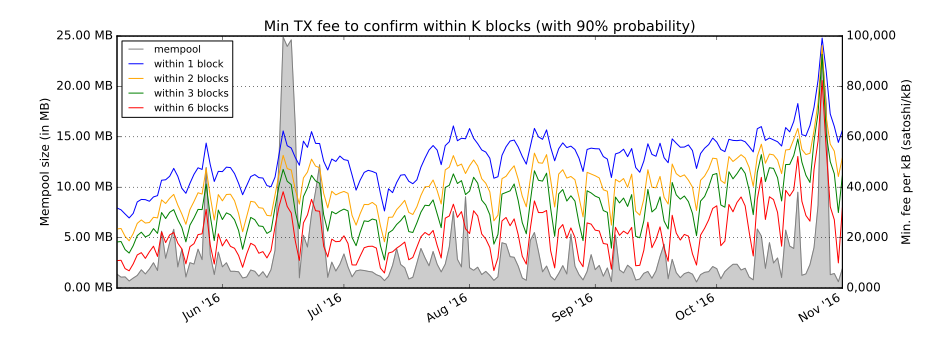
\includegraphics[width=2\columnwidth]{figs/txfee-estimates.eps}
	\vspace{-.9cm}
	\caption{This graphs shows the minimum transaction fee (in satoshi/kB) that guarantees a transaction will be included in the blockchain within $k$ blocks (for $k=1,2,3,6$) with 90\% probability (modeled using Feesim\cite{bitcoin-fees-github}). Fees tend to increase with contention for space in the Bitcoin ``mempool'' of unconfirmed transactions and transactions with higher fees get included in the blockchain faster. 1 satoshi = 0.00000001 BTC = $10^{-8}$ BTC and 1 kB = $10^3$ bytes.}
	\label{fig:fees}
\end{figure*}

We implemented a \Sys prototype in Java using the bitcoinj\cite{bitcoinj} library in 3000 lines of code, as measured with the \texttt{sloccount} tool.
Our code is available on GitHub: 

\begin{center}
\href{https://github.com/non-equivocation/catena-java}{\texttt{\footnotesize https://github.com/non-equivocation/catena-java}}
\end{center}

Our prototype implements a \Sys log server and a \Sys client, both operating as thin nodes on the Bitcoin network, but does not implement a header relay network (HRN).
Instead, in our first implementation, \Sys clients use only the Bitcoin P2P network to fetch both block headers and fetch \Sys transactions with their associated Merkle proofs.
In a future, more scalable implementation, we plan on fetching transactions and Merkle proofs from the log server and on using a header relay network for downloading block headers.
Next, we discuss our implementation and its internal API, which can be used to implement \Sys's API from \secref{sec:model:api}.

\subsection{\Sys Log Server}
The log server manages the statement key used to sign new \Sys statements (see \secref{sec:catena:design:transactions}) and a set of \emph{funding keys} used to ``re-fund'' a \Sys log (see \secref{sec:catena:design:refund}).
The server provides an $\mathsf{appendStatement(s)}$ API for issuing a statement $s$, which abstracts the Bitcoin layer away from applications.
Though currently not implemented, the server should ``re-fund'' the chain automatically assuming there are sufficient funds controlled by the funding keys.

\subsection{\Sys Log Client}
The client connects to the Bitcoin P2P network and sets a Bloom filter\cite{bloom} on all its connections to filter out irrelevant transactions.
This way, \Sys clients only receive server-issued \Sys transactions (see \secref{sec:background:bitcoin:thin}) and save orders of magnitude in bandwidth.
Recall that \Sys chains together transactions and clients verify this, thereby preventing malicious P2P nodes from equivocating about statements (see \secref{sec:catena:design:auditing}).
While additional bandwidth will be consumed by small blockchain reorganizations (see \secref{sec:catena:design:reorgs}), this amount should be negligible.

\Sys clients expose an $\mathsf{onStatementAppended(s)}$ API that notifies the higher level application of newly issued statements that have sufficient confirmations.
Applications are notified about statements in the order they were issued, making it easy to verify each statement for application-specific invariants (see \secref{sec:discussion:agnostic}).
If the \Sys log is caught equivocating, the \Sys client notifies the application via an $\mathsf{onEquivocation(s,s')}$ API that includes signatures on the two inconsistent statements $s$ and $s'$ and thus offers a publicly-verifiable non-repudiable proof of equivocation.

Certain applications might want to be made aware about the stability of Bitcoin's consensus.
For this, we provide an $\mathsf{onReorganize()}$ API that notifies applications about blockchain reorganizations with information about forks and the number of orphaned blocks.
Applications can use this information to infer whether the Bitcoin network is under attack, but we leave this to future work.

If bigger accidental or malicious forks should occur, they might unconfirm previously-confirmed \Sys transactions.
Even though such events are outside of our threat model, \Sys still notifies applications about statements that were unconfirmed via an $\mathsf{onStatementWithdrawn(s)}$ API so they can decide how to proceed.

\subsection{Costs and Overheads}

In this subsection, we discuss the financial cost of running a \Sys server, the overheads involved for clients and servers, and \Sys's scalability.

\subsubsection{Transaction Fees}
\label{sec:prototype:fees}
% https://bitcoinfees.21.co/#delay
% https://bitcoinfees.github.io/
% http://p2sh.info/dashboard/db/fee-estimation
Transaction fees in Bitcoin vary with contention for space in the blockchain (see \figref{fig:fees}) and so far have not been prohibitive for Bitcoin users.
For instance, Bitcoin transactions currently pay a fee of 70 satoshis per byte to get included in the blockchain within the next block\cite{bitcoin-fees-21co} (1 satoshi = $10^{-8}$ BTC).
For a 235-byte \Sys transaction that commits a statement consisting of a 256-bit SHA-256 hash, the fee would be 16,450 satoshis or 12 US cents per statement (on November 2016, 1 BTC = \$706.54).
If a statement is issued every 10 minutes, the cost per day would be less than 17.5 USD, which we believe is reasonable.
For example, this cost is not much higher than Keybase's cost\cite{keybase}, which issues statements less often (every 6 hours), paying a smaller fee of 10,000 satoshis or 7 US cents per transaction\cite{keybase-txs}.

\subsubsection{Overheads}
\label{sec:prototype:overheads}
\Sys's CPU overhead is insignificant.
A \Sys log server can issue at most one statement per Bitcoin block, so it only has to perform one signature every 10 minutes.
Similarly, \Sys clients only verify a transaction every 10 minutes for each log they audit, which adds virtually no overhead.
Finally, verifying the proof-of-work in block headers adds insignificant overhead.

\Sys clients need a small, constant amount of storage to recompute the Bitcoin difficulty and handle blockchain reorganizations.
To recompute the difficulty every 2016 blocks, \Sys clients and servers need to store the last 2016 block headers of the blockchain, which are 80 bytes each.
To prevent equivocation about withdrawn statements during blockchain reorganizations (see \secref{sec:catena:design:reorgs}), \Sys clients remember the past 100 statements issued by the server (no more than 80 bytes each due to \opret limits; see \secref{sec:background:bitcoin:opret}).
Here we assume that no Bitcoin fork, whether accidental or malicious, will be longer than 100 blocks.
Thus, \Sys's storage cost for both clients and servers is smaller than 200 KB.

\Sys demands a small amount of bandwidth from clients and a larger amount from servers who have to serve statements to clients.
First, servers and clients pay an initial cost to sync all the blockchain headers (currently \headerssize).
Servers and clients need to download all the headers so as to ensure the chain is sufficiently ``heavy'' and is thus the correct chain (see \secref{sec:background:bitcoin:consensus}).
Once this is done, \Sys clients need to sporadically connect to the header relay network to check for new block headers and connect to the log server to fetch new statements.
The required bandwidth for clients is less than 1 KB every 10 minutes: 600 bytes for statements and Merkle proofs and 80 bytes for each block header, possibly requested from multiple HRN nodes.
In contrast, the server needs bandwidth linear in the number of \Sys clients, since it serves every statement to each client.

\subsubsection{Scalability}
We believe \Sys can scale easily if the header relay network distributes block headers and the \Sys log server distributes statements and proofs.
However, our current implementation based on Bitcoin's P2P network will not scale beyond tens of thousands of \Sys clients without putting significant stress on Bitcoin.
As discussed in \secref{sec:catena:design:header-relay}, there simply aren't enough connections available in the Bitcoin network to support a large number of \Sys clients.
In addition, our current implementation relies on disk-intensive Bloom filtering (see \secref{sec:background:bitcoin:thin}).
We stress that these are current, surmountable limitations of Bitcoin that all \emph{thin} blockchain-based applications need to deal with, not just \Sys.

\subsection{Preventing Equivocation in CONIKS}
\label{sec:prototype:coniks}

\newcommand{\numlinessv}{66\xspace}
\newcommand{\numlinescl}{89\xspace}

To demonstrate \Sys's applicability to key transparency schemes, we modified CONIKS\cite{coniks} to publish directory digests in a \Sys log so as to prevent a malicious provider from equivocating about its \pkd.
Our modified CONIKS is as hard to fork as Bitcoin, which we believe makes CONIKS more resilient to attacks.
Our changes to CONIKS are minimal, consisting of \numlinessv new lines of code for the CONIKS server and \numlinescl new lines of code for the CONIKS test client. (We changed Java source files, project files and configuration files.)

A typical CONIKS provider advertises the root hash of a prefix Merkle tree periodically to CONIKS clients.
This root hash is signed and is referred to as a Signed Tree Root (STR).
To prevent impersonation, clients have to gossip STRs amongst themselves or with different providers.
Our modification of CONIKS removes the need for gossiping by witnessing STRs in the Bitcoin blockchain using a \Sys log.
This allows all CONIKS clients to agree on the same history of STRs.
We lowered the frequency at which providers publish STRs from once per minute to once per ten minutes to coincide with the frequency of Bitcoin blocks.
We also modified the CONIKS test client to listen for Bitcoin-witnessed STRs.
However, because the provided test client is not fully implemented to keep track of STRs, more changes to CONIKS, not \Sys, are needed to actually prevent equivocation.

\Sys does not change CONIKS's public-key distribution assumptions.
CONIKS assumes that clients have a way of obtaining the public keys of providers.
Similarly, our Bitcoin-witnessed CONIKS assumes that clients have a way of obtaining the ``public keys'' for the \Sys logs of providers.
Specifically, our ``public key'' is the log's genesis transaction (see \secref{sec:catena:design:genesis}).
We commit the old public key of the provider in the auxiliary data of the genesis transaction (see \secref{sec:model:api}).
CONIKS clients need this public key to verify CONIKS server replies to their queries.

\section{Discussion and Future Work}
\label{sec:discussion}

\setcounter{subsubsection}{0}
\subsubsection{Building \Sys on Top of Bitcoin}
We chose to design \Sys on top of Bitcoin because of Bitcoin's resilient proof-of-work consensus\cite{blockchainproto} and its real-world deployment.
This makes \Sys-enabled applications easy to deploy (no need to wait for trustworthy parties to come into existence) and expensive to attack (adversaries have to double spend in Bitcoin).
Still, it's important to note that Bitcoin's security as a ``black box'' consensus protocol remains an open problem.
For example, it can be difficult to dismiss externally-motivated adversaries who are well-incentivized to maliciously mine and double spend.
Finally, we note that \Sys could also be built on top of other blockchains such as Ethereum\cite{ethereum}, but we believe Bitcoin's security currently outmatches the security of all other blockchains.

% Regarding SPV, Peercoin doesn't seem to support it: https://talk.peercoin.net/t/does-peercoin-support-simplified-payment-verification/3697
% ...and neither Blackcoin nor NXT seem to mention anything about SPV.
In particular, we avoided Ethereum for a few reasons.
First, we believe Bitcoin is a more mature ecosystem to base applications on, given the many blockchain-based apps built on top of it\cite{blockstack,keybase,openassets,colu,coinspark}.
Second, Ethereum plans on transitioning to a proof-of-stake consensus algorithm\cite{proof-of-stake} called Casper\cite{ethereum-casper} that could change the trust assumptions behind thin nodes.
For instance, an additional assumption in Casper is that clients who are offline for too long can authenticate a list of ``bonded'' validators out-of-band\cite{ethereum-casper}.
Third, recent work shows that rational Ethereum miners have an incentive to skip verifying ``expensive'' blocks that other miners constructed maliciously\cite{consensuscomputer}.
In Bitcoin, such attacks are less practical since block verification does not involve executing arbitrarily complex smart contracts.

\subsubsection{Censorship}
\Sys's liveness depends on the censorship-resistance of the Bitcoin network.
Malicious miners can censor \Sys transactions and exclude them from the Bitcoin blockchain, which reduces the liveness of a \Sys log.
We stress, however, that Bitcoin's decentralized consensus does provide some degree of censorship-resistance by allowing \emph{any} honest miner to join the protocol, eventually resulting in an honest, non-censoring, majority.
We also stress that censorship attacks have not been observed in practice and we leave a more careful analysis of Bitcoin's censorship-resistance to future work.

\subsubsection{Historical Consistency}
\label{sec:discussion:agnostic}
\Sys is application-agnostic and does not guarantee application-specific \emph{internal consistency}\cite{ht} of statements, which needs to be checked at the application layer.
Instead, \Sys only guarantees \emph{historical consistency}\cite{ht} of statements, enabling applications to later check the correct semantics of statements.
As an example, \Sys ensures that all clients of a key transparency scheme such as Certificate Transparency (CT)\cite{ct} see the same history of signed tree heads (STHs).
However, clients still have to check the internal consistency of the STHs to detect impersonation.
For instance, Bob's client will want to make sure that across all STHs, his \pk has not been changed maliciously, and thus he hasn't been impersonated.

It is important to understand that without historical consistency, any guarantees of internal consistency are meaningless.
This is exactly why we designed \Sys. 
For instance, a malicious CT log server\cite{ct} can equivocate, giving Alice a signed tree head (STH) with her real \pk and a fake \pk for Bob, while giving Bob a different STH with his real \pk and a fake \pk for Alice.
Alice and Bob both verify their own STHs as being internally consistent and believe they were not impersonated.
However, because Alice and Bob have no historical consistency, they are looking at different STHs, which means the internal consistency guarantees they have are essentially useless.
In this case, Alice and Bob are being impersonated even though internal consistency tells them they are not.

\section{Related Work}
\label{sec:related-work}

% Tamper-evident logging
% ----------------------
Tamper-evident logging\cite{ht} allows auditors to ensure a log's correct behavior.
A \emph{history tree} is used to store events in the log, check their membership and prove that a new version of the log is consistent with a past version (i.e., no past events have been removed or modified).
Unfortunately, tamper-evident logging does not address equivocation attacks, assuming auditors can gossip to detect forks.
\Sys offers the same semantics as tamper-evident logging (\ie membership proofs, consistency proofs) but also prevents equivocation.
However, because the Bitcoin blockchain is implemented as a hash-chain, \Sys's membership and consistency proofs are linear, not logarithmic, in the log's size.
In practice, a \Sys log can commit root hashes of a history tree and prevent equivocation about the tree, while preserving logarithmic membership with respect to a root hash and logarithmic consistency proofs between two consecutive root hashes.

% Proofs of proofs of work
% ------------------------
Proofs of proofs of work (PPOW) \cite{ppow} enable thin clients to verify the ``weight'' of a blockchain (see \secref{sec:background:bitcoin:consensus}) by downloading only $O(\log{n})$ rather than all $n$ block headers.
Should Bitcoin adopt this interesting technique, \Sys clients could leverage it to download fewer block headers from the HRN.
First, we can leverage PPOWs to decrease the bootstrapping bandwidth of \Sys clients from $O(n)$ to $O(\log{n})$ when initially syncing with a blockchain of $n$ blocks.
Second, we can leverage PPOWs to skip downloading some of the block headers between two statements $s_i$ and $s_{i+1}$, should there be a large number of blocks between consecutive statements.
However, we cannot leverage PPOWs to skip downloading \Sys transactions and their corresponding block headers.
This is because \Sys clients need to verify that all \Sys transactions are chained correctly (see \secref{sec:catena:design:auditing}).

% uniquebits and CommitCoin
% -------------------------
Peter Todd's uniquebits\cite{uniquebits} allows users to publish signed hashes of arbitrary data in the Bitcoin blockchain for later auditing.
At a high level, the scheme commits the signed data $d$ and PGP fingerprint information about the signer by leveraging both ``Pay-to-Script Hash'' (P2SH) transactions\cite{bitcoin-p2sh-data} and ``fake'' \pks (see \secref{sec:background:bitcoin:opret}).
Unfortunately, uniquebits does not address the equivocation problem: the scheme cannot efficiently prevent a signer from publishing two pieces of data $d$ and $d'$ and equivocating to thin clients about which piece was signed.
Similarly, CommitCoin\cite{commitcoin} uses the Bitcoin blockchain to ``timestamp'' commitments and prove they were made at a certain time, but cannot efficiently prevent equivocation.

% Single-use seals
% ----------------
% Genesis TXN:
% https://blockchain.info/tx/b8b86d41647db9eb4fcb833cc685eb1264d7c3d2b8fb056551b3388e8c35a43b?show_adv=true
% Spends genesis, commits ID of next TXN (i.e., 5b6705437ced5cca8ec52cfb187e5d3270e067817c4fcd5a26755d4ceb4c010c)
% https://blockchain.info/tx/976e842f944b797352a111893d766ce1b3b211d987d31e764a424ee19de10fe5?show_adv=true
% Spends some random, unrelated transaction
% https://blockchain.info/tx/5b6705437ced5cca8ec52cfb187e5d3270e067817c4fcd5a26755d4ceb4c010c?show_adv=true
% Spends transaction above, , commits ID of next TXN
% https://blockchain.info/tx/19c2aa81cf6a0bf7d1f20810ca72baac44cb2532d765e162b0d58b4e050ff3af?show_adv=true
Concomitant with the publication of our online version of \Sys\cite{catena-eprint}, Peter Todd independently proposed a Bitcoin-based log that prevents equivocation using \emph{single-use seals}\cite{single-use-seals}.
Single-use seals generalize the concept of spending a transaction output in Bitcoin while committing some arbitrary data in the process.
The transaction output waiting to be spent is the \emph{identifier} of the single-use seal, while the transaction that spends that output and commits some arbitrary data (see \secref{sec:background:bitcoin:opret}) is known as the \emph{closing transaction}.
Importantly, when a seal is ``closed'' by spending its output via a closing transaction, another seal can be specified as the arbitrary data in that transaction.
This is similar to how, in \Sys, a new transaction spends the previous transaction's continuation output (equivalent to ``closing a seal'') and creates a new continuation output (equivalent to specifying a new seal).

As opposed to \Sys, single-use seals provide a certain degree of censorship-resistance because the identifier of the next seal can be hidden from miners by committing to it in the closing transaction.
In contrast, with \Sys, the next continuation output (see \secref{sec:catena:design:transactions}) is always public and known by miners, so they can censor transactions that try to spend it.
However, \Sys is more efficient than single-use seals, since each statement requires a single transaction to be posted on the blockchain, while single-use seals require two transactions (one transaction for the seal's identifier plus another closing transaction).
Furthermore, although thin client verification of a log would be possible with single-use seals, the details of this are never considered in depth\cite{single-use-seals}, a contribution that \Sys makes.
Finally, to the best of our knowledge, single-use seals have not been implemented yet, making \Sys the first implementation of an efficient Bitcoin-based log.

% Keybase
% -------
Keybase\cite{keybase} and Blockstack\cite{blockstack,virtualchain} use the Bitcoin blockchain to prevent equivocation but do so inefficiently, requiring clients to run a full Bitcoin node.
Keybase periodically publishes the Merkle root of its \pkd by committing it in transactions signed under a fixed \pk known by Keybase clients\cite{keybase-txs}.
Specifically, Keybase stores the Merkle root in the transaction's output as a ``fake'' \pk (see \secref{sec:background:bitcoin:opret}).
Unfortunately, this approach does not allow clients to efficiently and correctly obtain all Keybase-issued transactions using Bloom filtering (see \secref{sec:background:bitcoin:thin}).
This is because Bitcoin P2P nodes can selectively hide transactions from clients and show different transactions to different users, thus equivocating about the Keybase directory (see \secref{sec:catena:design:auditing}).
In \Sys, a new transaction always spends the previous one, creating a unique chain due to the difficulty of double spending.
As a result, all \Sys clients see the same history of transactions, implicitly agreeing on the history of statements.

% Blockstack
% ----------
In Blockstack\cite{blockstack}, users submit their own operations (e.g., ``register \pk'' or ``update \pk'') to the Bitcoin blockchain by creating transactions that include these operations in an \opret output.
Blockstack nodes download the full Bitcoin blockchain and filter these Blockstack-specific transactions (recognized via a magic byte in the \opret data), accumulating the Blockstack operations into a \emph{consensus hash}\cite{blockstack}.
Importantly, thin clients can query Blockstack nodes for \pks (\eg ``look up Alice's \pk'') and authenticate their responses against a consensus hash.
Unfortunately, because thin clients cannot download the entire blockchain, they would have to obtain consensus hashes from a trusted entity which, if compromised, could equivocate about these hashes.
In this sense, \Sys could make equivocation about consensus hashes as hard as forking Bitcoin, thereby increasing Blockstack's thin client security (discussed in \secref{sec:background:motivation:blockchain-transparency}).

% Colored coins
% -------------
Coin coloring schemes \cite{colu,openassets,coinspark} leverage the Bitcoin blockchain to enable the secure issuance and transfer of assets different than bitcoins, such as smart property, stocks or bonds\cite{coloredcoinsoverview}.
The key idea is that a set of coins locked in an output can be assigned a static color which can be correctly maintained as those coins change hands.
To prevent double spending of colored coins, coloring schemes also leverage Bitcoin's security against double spends along with some additional verification by ``color-aware'' wallets.
The overhead of these schemes is similar to \Sys's, since ``color-aware'' (thin) wallets only need to keep track of transactions that affect an asset (e.g., reassigned ownership).

Coin coloring schemes and \Sys both rely on the difficulty of double spending but do so to solve slightly different problems.
Specifically, while coin coloring schemes prevent equivocation about the never-changing color of a coin, \Sys prevents equivocation about an ever-growing log of statements.
While some coloring schemes support committing arbitrary data in their transactions\cite{coloredcoins-metadata} and could be adapted to prevent equivocation, to the best of our knowledge, this has not yet been done.
Thus, we believe \Sys to be the first system that solves the equivocation problem efficiently using Bitcoin.

% Coins on fire!
% --------------------------
Non-equivocation contracts\cite{liarliar} disincentivize equivocation by penalizing it with monetary loss.
Specifically, if an authority equivocates, its Bitcoin secret key, which locks some funds, is implicitly revealed via a mechanism similar to double-authentication-preventing signatures (DAPS)\cite{daps}.
As a result, anybody who detects equivocation can spend those funds.
The advantage of non-equivocation contracts is that statements are not included in the Bitcoin blockchain so they can be issued faster than in \Sys.
This enables interesting applications, such as asynchronous payment channels\cite{liarliar}, which are not possible with \Sys.
However, as opposed to \Sys, non-equivocation contracts only disincentivize equivocation and do not necessarily prevent it.
For example, an outsider who steals the authority's secret key and wants to harm the authority is actually incentivized to equivocate and can easily do so.
With \Sys, even with a stolen secret key, an outsider cannot equivocate without forking the Bitcoin blockchain.

% CoSi
% ----
CoSi\cite{cosi} prevents equivocation by requiring a threshold number of ``witnesses'' to also verify and sign an authority's statements.
Depending on the application, these witnesses could also check the internal consistency of statements (see \secref{sec:discussion:agnostic}). 
In contrast, \Sys prevents equivocation by assuming its authority, Bitcoin, is trustworthy, without relying too much on the header relay network (HRN) to keep it honest (see \secref{sec:attacks:hrn}).
Both CoSi and \Sys make assumptions about connectivity of participants.
CoSi requires a relatively well-connected set of witnesses for its tree broadcast scheme while \Sys requires the Bitcoin P2P network not to be easily partitioned.
One drawback of CoSi is that it requires an admission control process for witnesses to prevent Sybil attacks\cite{sybil}.
As a result, finding witnesses who are reputable, trustworthy entities could be hard.
In contrast, \Sys could be easier to deploy since it only relies on the Bitcoin blockchain as a single trustworthy witness and on a header relay network that can be bootstrapped using existing blockchain explorers (see \secref{sec:catena:design:header-relay}).

Like CoSi, \Sys can offer both ``proactive'' and ``retroactive'' security \cite{cosi}.
In particular, \Sys can be used retroactively by clients to validate previously accepted statements, or it can be used proactively before accepting a statement as valid.
Unlike CoSi, \Sys suffers a higher delay when used proactively because clients have to wait for sufficient confirmations before accepting a statement.
This is a cost \Sys pays for using a decentralized consensus network as its only witness.
However, we stress that not all applications care about this cost.
In particular, \Sys is suitable for key transparency schemes, Tor directory servers and software transparency schemes, which all perform batching and update their state infrequently.

% Key transparency
% ----------------
Key transparency schemes can detect equivocation using gossip amongst users\cite{ctgossip,ect,coniks,dtki}, gossip between users and trusted validators\cite{aki}, federated trust\cite{coniks}, any-trust assumptions\cite{arpki} or non-collusion between actors\cite{arpki, aki}.
\Sys instead relies on the resilience of Bitcoin's proof-of-work consensus to prevent, not just detect, equivocation.
Our approach can provide proactive security\cite{cosi} at the cost of publishing new statements every 10 minutes with an average 60-minute confirmation latency (if clients wait for 6 confirmations).
Alternatively, \Sys can provide retroactive security with no latency.
We believe \Sys can strengthen key transparency schemes because it enables anyone to audit efficiently for non-equivocation.
We also believe \Sys's approach to non-equivocation is simpler and more trustworthy due to the decentralized nature of Bitcoin's consensus protocol.

% EthiKS
% ------
% 1 gas is usually 20 gweis
% 1 gwei is 0.000000001 = 10^-9 ETH
% 1 gas = 20 gwei = 0.0000 0002 ETH = 2 * 10^-8 ETH
% 1 ETH = 12 USD
% 1 gas = 2 * 10^-8 * 12 USD
%
% EthIKS costs|
% ------------*------------*----------------------------
% Create tree | 367535 gas | 0.01837675 USD = 1.8 cents
% Insert user | 42042 gas  | 0.0021021 USD = .2 cents
% Update user | 12042 gas  | 0.0006021 USD = .06 cents
EthIKS\cite{ethiks} uses the Ethereum blockchain\cite{ethereum} to prevent equivocation in CONIKS\cite{coniks}, a key transparency scheme that enables users to efficiently monitor their own public key bindings.
EthIKS implements CONIKS as a ``smart contract'' in the Ethereum blockchain and relies on Ethereum miners to enforce CONIKS security invariants.
Like \Sys, EthIKS also efficiently leverages proof-of-work consensus within a cryptocurrency to prevent equivocation in the log.
However, different from \Sys, EthIKS guarantees internal consistency (see \secref{sec:discussion:agnostic}) of the CONIKS log, though this comes at the expense of additional Ethereum transaction fees paid by the EthIKS log server\cite{ethiks}.
In contrast, \Sys clients have to check each log statement for internal consistency themselves, incurring an overhead linear in the number of statements in the log.
For certain applications where internal consistency checks are not expensive (e.g., monitoring your own binding in a \pkd) and minimizing server costs is a priority, \Sys could be better suited.
However, when server costs are not a concern (e.g., costs can be shifted to users), Ethereum-based approaches like EthIKS could be better suited.


\section{Conclusion}
\label{sec:conclusion}
We design and implement \Sys, an append-only log that is as hard to fork as the Bitcoin blockchain but efficient to verify by thin clients such as mobile phones.
Specifically, in \Sys, an attacker can equivocate if and only if he can double spend Bitcoin transactions, which is notoriously difficult due to Bitcoin's proof-of-work consensus.
The key idea behind \Sys is to chain \opret transactions together by having a new transaction spend the previous one, making equivocation in the log as hard as double spending in Bitcoin.

\Sys can be used to prevent equivocation in key transparency schemes, paving the way for more trustworthy \pkds.
\Sys can also be used as a public log for Tor Consensus Transparency\cite{tortransparency}, as a software transparency scheme to prevent malicious software updates or as a consensus log for mutually distrusting participants.
\Sys's overheads are small.
Clients only need to download 80-byte block headers and 600-byte statements, a significant improvement over previous blockchain-based transparency schemes\cite{keybase,virtualchain,blockstack} which currently require auditors to download \blockchainsize of blockchain data\cite{bitcoin-size}.
We develop a prototype of \Sys in Java and apply it to CONIKS, a key transparency scheme, demonstrating \Sys's feasibility.
Next, we plan on extending our prototype to scale for popular applications.

Our main reason for designing \Sys is to prevent equivocation in compromised online services.
In that sense, we believe \Sys can bring Bitcoin's non-equivocation guarantees to many important applications today.
In particular, we hope \Sys can be adopted by secure messaging apps such as Signal\cite{signal} or \pkds such as Keybase\cite{keybase}, giving end users stronger guarantees about non-equivocation.

\section*{Acknowledgment}
We would like to thank our shepherd, Jay Lorch, and the anonymous reviewers for their insightful comments that helped improve this paper.
We would also like to thank Conner Fromknecht, Albert Kwon, Ilia Lebedev, Neha Narula, Ling Ren and the MIT Digital Currency Initiative for the many productive conversations that shaped and improved this work.

%\nocite{*} % when you compile, tells you if you haven't cited any items in your .bib file, but needs \usepackage{refcheck}

\bibliographystyle{IEEEtran/bibtex/IEEEtran}
\bibliography{IEEEtran/bibtex/IEEEfull,references}
%\bibliographystyle{IEEEtrancr/IEEEtranBST/IEEEtran}
%\bibliography{IEEEtrancr/IEEEtranBST/IEEEfull,references}
%\printbibliography % for biblatex

%\appendix
